\documentclass[11pt,a4paper]{article}
\usepackage[utf8]{inputenc}
\usepackage[T1]{fontenc}
\usepackage{babel}
\babelprovide[import,main]{spanish}
\usepackage[margin=2.5cm]{geometry}
\usepackage{amsmath,amssymb,booktabs,tabularx,microtype}
\usepackage{tikz}
\usetikzlibrary{arrows.meta,positioning}
\usepackage[hidelinks]{hyperref}
\usepackage{xurl}
\newcommand{\Wi}{W_i}
\newcommand{\ind}{\mathbf{1}}
\newcommand{\E}{\mathbb{E}}
\newcommand{\loss}{\mathcal{L}}
\newcommand{\KB}{\mathcal{K}}
\newcommand{\sg}{\operatorname{sg}}
\setlength{\emergencystretch}{2em}
\title{Matrix--NCM: aprendizaje de campos semánticos contextuales\newline
mediante restricciones lógicas y ruteo reflexivo}
\author{Borrador de trabajo --- autoría y afiliación por completar}
\date{23 de octubre de 2026 \quad Versión 0.1}

\begin{document}
\maketitle
\begin{abstract}
Proponemos aprender representaciones cuyo objetivo sea el campo semántico
indicado por una ocurrencia textual bajo un contexto. El contexto combina
dimensiones transversales, como tema, país, registro y función retórica; su
organización jerárquica constituye una decisión de representación, no una
taxonomía universal del conocimiento. Matrix aporta mundos lógicos locales,
distinciones entre verdad, aplicabilidad y discriminación, y mecanismos para
representar relaciones entre contextos. Formulamos una extensión en la que el
ruteo también se expresa como conocimiento evaluable y aprendible. Next-Concept
Modeling (NCM) proporciona una posible base de cuantización multiescala sobre la
cual entrenar esta representación. Presentamos objetivos de grounding, lógica,
sentido y organización contextual, junto con un protocolo de datos RDF--texto.
Un experimento sintético de 560 consultas muestra que condicionar antes de la
cuantización permite resolver cambios contextuales que un modelo sin contexto
no distingue. Este resultado verifica un mecanismo limitado: no demuestra
aprendizaje de campos semánticos ni de jerarquías. El documento separa los
componentes existentes, la propuesta matemática y las hipótesis pendientes.
\end{abstract}

\section{Introducción}
Un signo textual no determina por sí solo qué se está diciendo. Una ocurrencia
de una palabra participa en relaciones que dependen del texto, del ámbito de
uso y de las distinciones disponibles. Incluso un embedding sensible al contexto
no garantiza que esas relaciones puedan evaluarse como un sistema lógico ni que
su organización resulte explícita y revisable.

La propuesta parte de cuatro compromisos. Primero, el objetivo semántico de
predicción es el campo al que apunta una ocurrencia, no su identidad ortográfica.
Segundo, un campo admite múltiples dimensiones transversales. Tercero, las
jerarquías organizan el acceso contextual a un grafo relacional y pueden variar
sin que cambien los hechos representados. Cuarto, las decisiones de ruteo son
también relaciones que el sistema puede representar, evaluar y aprender.

Matrix ofrece fundamentos y componentes operacionales para expresar estos
compromisos. La integración propuesta busca que intervengan en el aprendizaje
de la representación, en lugar de limitarse a evaluar un embedding congelado.
NCM se considera una implementación posible del soporte discreto multiescala,
sin identificar de antemano sus códigos con conceptos lógicos.

Este trabajo es un borrador de arquitectura con evidencia preliminar. Sus
contribuciones propuestas son una formulación contextual del objetivo semántico,
un tratamiento reflexivo del ruteo y un criterio de aprendizaje que separa
consistencia, aplicabilidad y coste de organización. No se reivindica prioridad
sobre el aprendizaje neuro-simbólico en general ni una arquitectura completa ya
validada experimentalmente.

\section{Fundamentos y antecedentes}
\subsection{Del signo a su función contextual}
La documentación de Matrix desarrolla la distinción entre signo y símbolo:
la forma perceptible se diferencia de su función dentro de relaciones lógicas.
El documento operacional sobre contexto sostiene que el referente se delimita
por las restricciones que sobreviven a sucesivos contextos. Esta es la base
conceptual del objetivo de campo semántico usado aquí\cite{matrix}.

País, género discursivo, tema y función retórica no son necesariamente niveles
de un árbol. Un tratado puede ser académico, referirse a un país y contener una
objeción sobre un tema determinado. Esas dimensiones se cruzan. Asimismo, una
proposición admisible en una fábula puede resultar inaplicable en un mundo
botánico especificado, sin que eso establezca una prohibición universal sobre
el uso metafórico del lenguaje.

\subsection{Representaciones discretas y supervisión lógica}
VQ-VAE permite aprender códigos discretos mediante cuantización de vectores y
una aproximación al gradiente\cite{vqvae}. NCM utiliza una representación
residual multiescala y un generador que predice niveles de grueso a fino, con
posiciones de cada nivel generadas en paralelo\cite{ncm}. Esta estructura
computacional ofrece una base para estudiar refinamientos contextuales; no
establece que un nivel corresponda a una categoría ontológica.

Semantic Loss conecta probabilidades neuronales con satisfacción de fórmulas
booleanas\cite{semanticloss}. Logic Tensor Networks utiliza una lógica
diferenciable para integrar aprendizaje y razonamiento\cite{ltn}. La propuesta
presente se sitúa en esta línea, pero estudia conjuntamente la aplicabilidad
contextual y la organización del acceso a los campos. La novedad específica de
esa combinación requiere comparación bibliográfica y experimental adicional.

\section{Objetos y semántica operacional}
\subsection{Ocurrencias, campos y contexto}
Sea $x$ un texto, $o$ una ocurrencia o span de $x$, y $c_{\rm obs}$ el contexto
disponible para la tarea. Una ocurrencia no tiene que coincidir con un token
subword: varias unidades de superficie pueden indicar un mismo referente.
Distinguimos el campo semántico $f$, su representación continua $z$, los códigos
cuantizados $q$ y los tokens de superficie. Ninguna igualdad entre esos cuatro
objetos se presupone.

Para hacer entrenable el objetivo, se propone un conjunto finito de candidatos
$\mathcal{F}$ en cada ejemplo. Un candidato puede denotar una región de
posibilidades compatible con restricciones, no necesariamente una entidad única.
El objetivo es
\begin{equation}
 p_\theta(f\mid o,x,c), \qquad f\in\mathcal{F}.
\end{equation}
La elección de candidatos y su equivalencia entre contextos forman parte del
problema de grounding. La distribución por sí sola no define una ontología.

Sea $\gamma$ una organización contextual: selección de dimensiones, mundos y
relaciones de acceso. Un modelo puede inferirla cuando no esté dada:
\begin{equation}\label{eq:joint}
 p_{\theta,\phi}(f,\gamma\mid o,x,c_{\rm obs})=
 p_\phi(\gamma\mid o,x,c_{\rm obs})\,
 p_\theta(f\mid o,x,c_{\rm obs},\gamma).
\end{equation}
Esta es una factorización propuesta. En comprensión, $x$ puede ser el texto
completo; en generación, se sustituye por la información disponible en ese
paso. Usar el texto futuro durante inferencia produciría fuga de información.

\subsection{Mundos locales: verdad, sentido y discriminación}
Un espacio local se describe mediante ejes y una relación,
$L_i=(A_i,B_i,R_i,C_i)$, donde $C_i$ recoge restricciones del espacio. Un juego
$W_i$ incorpora el estado y su contexto $c_i$. Para una proposición admisible
$p=(R_i,a,b)$, distinguimos:
\begin{align}
 V_i(p)&\in\{\mathrm{true},\mathrm{false},\mathrm{unknown}\},\\
 S_i(p)&\in\{\mathrm{sinnvoll},\mathrm{sinnlos},\mathrm{unsinnig}\}.
\end{align}
En esta propuesta, la supervisión binaria de aplicabilidad se obtiene como
$a_i(p)=\ind[S_i(p)\neq\mathrm{unsinnig}]$. No se identifica desconocido con
falso, ni se identifica ausencia de poder discriminativo con inaplicabilidad.

La implementación puede devolver un sentido almacenado y, por otra ruta,
calcular el carácter no discriminativo de una columna universal. Por ello,
la integración debe fijar un contrato de evaluación; no basta entrenar sobre
la cadena textual que devuelve cualquier operación. $D_i$ designa aquí la
capacidad discriminativa de una elección contextual, sin suponer que exista
una matriz universal entrenable con ese nombre en el runtime actual.

\subsection{Jerarquías como decisiones de organización}
El grafo de hechos no necesita poseer una única raíz. Una organización $\gamma$
selecciona recorridos y factorizaciones que permiten acceder a sus relaciones.
Colocar perros dentro de una rama dedicada a frutas, en un contexto ordinario
explícitamente tipado, puede introducir numerosos cruces inaplicables. Una
organización alternativa puede preservar los hechos con menos celdas inútiles.

Esto no implica minimizar toda entropía: una pregunta que divide candidatos
equilibradamente puede aportar más información. Deben distinguirse incertidumbre
residual, ganancia informativa y coste de almacenamiento o consulta. Tampoco
toda celda no observada es un \emph{don't-care}: puede ser una coordenada
admisible cuyo valor todavía se desconoce.

\subsection{Ruteo reflexivo}
Las organizaciones pueden describirse mediante proposiciones como
\begin{equation}
 (\mathrm{routes\_to},c_i,W_j),\qquad
 (\mathrm{selects},c_i,d_k),
\end{equation}
donde $d_k$ es una dimensión candidata. Esas proposiciones se evalúan en juegos
de nivel meta, con sus propias condiciones de sentido y verdad. El mismo
formalismo representa hechos del dominio y decisiones sobre cómo consultarlos.

Esto permite proponer rutas mediante una red y evaluarlas simbólicamente. No
elimina la necesidad de un ejecutor ni de un punto de arranque: el prototipo
futuro debe usar un conjunto finito de candidatos, un presupuesto de profundidad
y reglas explícitas para ciclos. La equivalencia de dos organizaciones debe
comprobarse por las consultas que preservan, no por la igualdad de sus rutas.

\section{Arquitectura propuesta e integración con NCM}
\begin{figure}[t]
\centering
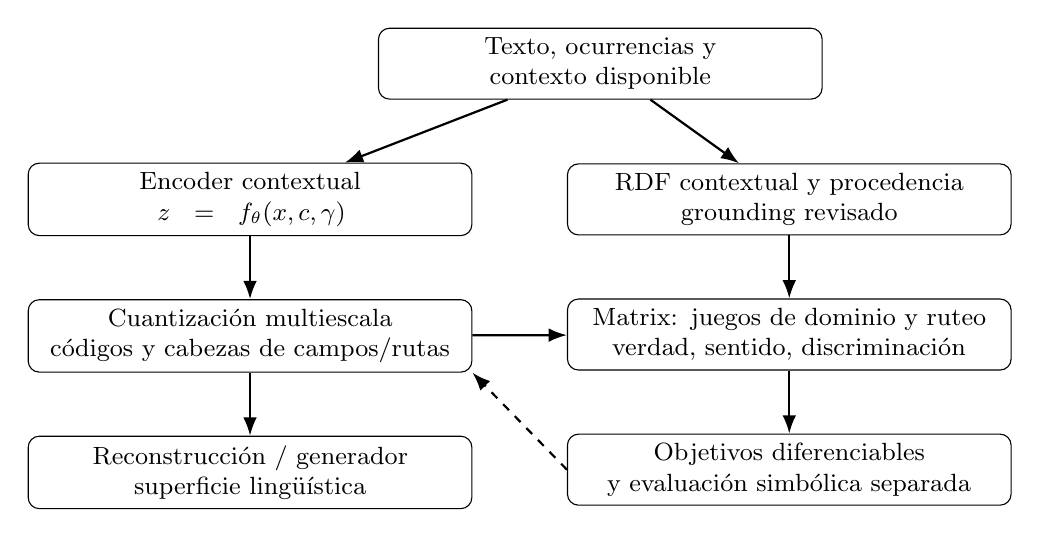
\begin{tikzpicture}[node distance=8mm and 12mm,
 box/.style={draw,rounded corners,align=center,text width=5.4cm,minimum height=9mm,font=\small},
 arr/.style={-{Latex},thick}]
\node[box] (text) {Texto, ocurrencias y contexto disponible};
\node[box,below left=of text,xshift=24mm] (enc) {Encoder contextual\\$z=f_\theta(x,c,\gamma)$};
\node[box,right=of enc] (rdf) {RDF contextual y procedencia\\grounding revisado};
\node[box,below=of enc] (vq) {Cuantización multiescala\\códigos y cabezas de campos/rutas};
\node[box,below=of rdf] (mat) {Matrix: juegos de dominio y ruteo\\verdad, sentido, discriminación};
\node[box,below=of vq] (dec) {Reconstrucción / generador\\superficie lingüística};
\node[box,below=of mat] (loss) {Objetivos diferenciables\\y evaluación simbólica separada};
\draw[arr] (text)--(enc); \draw[arr] (text)--(rdf);
\draw[arr] (enc)--(vq); \draw[arr] (rdf)--(mat);
\draw[arr] (vq)--(dec); \draw[arr] (vq)--(mat);
\draw[arr] (mat)--(loss); \draw[arr,dashed] (loss.west)--(vq.south east);
\end{tikzpicture}
\caption{Arquitectura propuesta. El gradiente procede de pérdidas sobre salidas
neuronales; ejecutar el kernel discreto no crea por sí mismo una ruta diferenciable.
La extracción general de RDF y el aprendizaje del ruteo siguen pendientes.}
\end{figure}

\subsection{Condicionamiento antes de cuantizar}
Proponemos que la representación dependa del contexto antes de asignar códigos:
\begin{equation}
 z=f_\theta(x,c_{\rm obs},\gamma),\qquad
 q^{1:K}=Q(z),\qquad \hat{x}=d_\psi(q^{1:K},c_{\rm obs}).
\end{equation}
El código no recibe una definición fija como ``721 = árbol''. Su función debe
medirse mediante las relaciones, campos y restricciones que permite recuperar.
La reconstrucción ayuda a preservar contenido lingüístico, pero por sí sola no
garantiza alineación semántica.

En el código NCM inspeccionado, la asignación discreta usa vecinos próximos;
la salida aplica un estimador straight-through y los codebooks se actualizan
mediante EMA. Esquemáticamente,
\begin{equation}
 z_{\rm ST}=z+\sg[Q(z)-z].
\end{equation}
La pasada directa utiliza vectores cuantizados y la derivada respecto de $z$
se aproxima por la identidad. Las pérdidas añadidas pueden modificar el encoder;
eso no significa que Adam optimice directamente los codebooks. Varias funciones
de conveniencia de inferencia están bajo \texttt{no\_grad}; el entrenamiento debe
usar la ruta forward apropiada\cite{ncmcode}.

\subsection{Cómo se predicen contextos y campos hacia abajo}
Un esquema explícito de descenso mantiene el estado
$h_\ell=(q^{<\ell},\gamma_{<\ell},c_{\rm obs})$.
Primero selecciona una decisión contextual $r_\ell$ y después produce los códigos
del nivel bajo esa decisión:
\begin{align}
 r_\ell&\sim p_\phi(r_\ell\mid h_\ell),\\
 q^\ell&\sim p_\theta(q^\ell\mid h_\ell,r_\ell),\\
 \gamma_{\leq\ell}&=\operatorname{update}(\gamma_{<\ell},r_\ell).
\end{align}
Una cabeza de grounding interpreta los códigos como una distribución de campos,
$p_\eta(f\mid q^{\leq\ell},\gamma_{\leq\ell},c_{\rm obs})$. Así, la ruta puede
elegir qué distinción conviene hacer y el campo predicho queda condicionado por
esa elección. En un primer modelo, $r_\ell$ seleccionaría entre alternativas
enumeradas; generar nuevos símbolos o dimensiones sería una extensión posterior.

El índice multiescala $\ell$ es computacional. No exige que primero se prediga
país, después tema y luego especie. Tampoco se supone una correspondencia uno
a uno entre niveles VQ y niveles de navegación. La predicción paralela dentro
de un nivel sólo se conserva si las decisiones de ruteo no introducen dependencias
secuenciales adicionales. El ahorro de inferencia debe medirse de nuevo.

Si una decisión sólo refina una dimensión, puede exigirse que su región candidata
sea un subconjunto de la anterior. Si cambia el marco de interpretación, esa
inclusión no es válida automáticamente: hace falta una proyección entre contextos.
La similitud vectorial no constituye por sí sola una identidad de referentes.

\section{Objetivos de aprendizaje}
\subsection{Grounding y aplicabilidad}
Para ocurrencias con un campo supervisado $f^*$,
\begin{equation}
 \loss_G=-\sum_{o\in\mathcal{O}_{\rm lab}} w_o
 \log p_\eta(f^*_o\mid q_o,c_o,\gamma_o).
\end{equation}
Cuando varias regiones son compatibles, debe supervisarse un conjunto o una
distribución, evitando imponer una identidad no justificada. Los pesos $w_o$
representan confianza documentada en el alineamiento, no certeza automática
del extractor.

Sean $s_p$ la probabilidad neuronal de aplicabilidad, $v_p$ la de verdad,
$a_p$ la etiqueta de aplicabilidad y $k_p$ el indicador de verdad observada.
Con normalización por ejemplos supervisados:
\begin{align}
 \loss_S&=\sum_{p\in\mathcal{P}_{S}}\operatorname{BCE}(s_p,a_p),\\
 \loss_V&=\sum_{p\in\mathcal{P}} a_p k_p\,
             \operatorname{BCE}(v_p,V(p)).
\end{align}
Las máscaras $a_p,k_p$ de supervisión son externas al predictor en esta etapa:
el modelo no puede evitar una penalización de verdad declarando que el ejemplo
es inaplicable. Los valores desconocidos no reciben una etiqueta falsa.

\subsection{Restricciones lógicas}
Para una fórmula $\varphi$ sobre átomos aplicables distintos y probabilidades
$v_1,\ldots,v_m$, una opción es la pérdida semántica\cite{semanticloss}:
\begin{equation}
 \loss_{\rm logic}(\varphi)=
 -\log\left[\sum_{\mathbf{b}\models\varphi}
       \prod_{j=1}^{m}v_j^{b_j}(1-v_j)^{1-b_j}\right].
\end{equation}
La expresión asume una distribución Bernoulli factorizada sobre los átomos;
sus repeticiones dentro de una fórmula comparten variable. La enumeración
directa crece exponencialmente, por lo que un sistema mayor necesita compilación
o restricciones locales. Para dos átomos distintos $A\Rightarrow B$ se reduce a
$-\log[1-v_A(1-v_B)]$.

El ámbito de una regla debe fijar dónde es aplicable. Una fórmula cuyo átomo
queda fuera de contexto no se transforma arbitrariamente en falsa. Conviene
separar restricciones sobre sentido de restricciones sobre verdad dentro de un
mundo. La satisfacción blanda tampoco garantiza que una muestra discreta sea
válida: se conserva la evaluación exacta como métrica independiente.

\subsection{Coste de organización y aprendizaje de rutas}
Una posible función a minimizar sobre organizaciones candidatas es
\begin{equation}\label{eq:cost}
 J(\gamma)=\alpha C_{\rm cells}(\gamma)
 +\beta C_{\rm inap}(\gamma)
 +\delta C_{\rm query}(\gamma)
 +\epsilon H(F\mid\mathcal{A}_\gamma)
 +\zeta C_{\rm uncovered}(\gamma),
\end{equation}
con términos normalizados. $C_{\rm cells}$ mide coste representacional;
$C_{\rm inap}$ cuenta cruces inaplicables según un contrato de referencia;
$C_{\rm query}$ mide coste de recorrido; $\mathcal{A}_\gamma$ son respuestas a
distinciones seleccionadas; y $C_{\rm uncovered}$ penaliza hechos o consultas
que la organización deja de cubrir. Comparar las alternativas exige la misma
distribución de consultas. No se acepta obtener un buen coste borrando evidencia.

La ecuación~\ref{eq:cost} es una propuesta, no la función implementada por Matrix.
El módulo actual de partición compara alternativas suministradas principalmente
por número de celdas y reutilización del término medio.

Para un conjunto pequeño de organizaciones, se puede calcular exactamente
\begin{equation}
 \loss_R=\sum_{\gamma\in\Gamma}
 p_\phi(\gamma\mid x,c_{\rm obs})J(\gamma).
\end{equation}
Aunque $J$ se evalúe discretamente, esta suma es diferenciable respecto de sus
probabilidades. Para espacios mayores se necesitarían propuestas y estimadores
por muestreo, o relajaciones cuyo sesgo se evalúe. Las reglas de ruteo se validan
además en juegos meta. La estructura propuesta por el modelo no puede ser la
única autoridad que certifique su propia corrección.

\subsection{Objetivo conjunto y calendario}
\begin{equation}
 \loss=\loss_{\rm rec}+\lambda_Q\loss_{\rm VQ}
 +\lambda_G\loss_G+\lambda_V\loss_V+\lambda_S\loss_S
 +\lambda_L\loss_{\rm logic}+\lambda_R\loss_R.
\end{equation}
Cada término corresponde a una señal distinta. En particular, enseñar verdad
de siete predicados no equivale a supervisar campos semánticos de ocurrencias.
Se propone comenzar con tokenizer y cabezas bajo rutas conocidas, incorporar
después elección entre rutas y finalmente adaptar el generador. Si cambia el
tokenizer, deben recodificarse sus objetivos y revisarse las cabezas del generador
que dependen de los codebooks. El entrenamiento conjunto completo queda abierto.

\section{Datos RDF--texto y construcción de supervisión}
WebNLG empareja conjuntos de triples RDF con realizaciones textuales y constituye
un punto de partida para grounding y generación\cite{webnlg}. WebNLG+ incorpora
las direcciones texto a RDF y RDF a texto en inglés y ruso\cite{webnlgplus}.
Estos recursos no aportan automáticamente todas las dimensiones contextuales
ni etiquetas de absurdo local requeridas por la propuesta.

El contrato de ejemplo propuesto es
\begin{equation}
 d=(x,\mathcal{O},G,c_{\rm obs},\Pi,\KB,\mathcal{Y}),
\end{equation}
donde $G$ es el grafo, $\Pi$ conserva procedencia y alineamientos, $\KB$ contiene
restricciones y $\mathcal{Y}$ etiquetas observadas con sus máscaras. Deben
preservarse las URIs completas, la fuente, la negación y el alcance contextual.
Turtle es una sintaxis de serialización; las etiquetas adicionales de sentido
pertenecen al esquema del experimento, no aparecen por usar esa sintaxis.

La construcción del dataset requiere: alinear spans y proposiciones; compilar
juegos locales por contexto y relación; registrar restricciones y su procedencia;
generar alternativas contextuales controladas; y verificar la preservación de
consultas bajo particiones alternativas. Los negativos deben justificarse por
restricciones locales o anotación. Un triple ausente no es un negativo, y los
dominios/rangos RDF no deben tratarse sin más como validadores de un mundo cerrado.

Para probar las transversales se necesitan pares con el mismo signo y distinto
contexto, paráfrasis con el mismo referente y cambios retóricos que no alteren
los hechos. Las particiones de evaluación deben separar entidades y, en pruebas
adicionales, combinaciones de dimensiones, fuentes y plantillas. El subconjunto
contrafáctico debe marcarse como construido; no se presenta como dato original
de WebNLG. La calidad del extractor se evalúa separadamente del modelo semántico.

\section{Evidencia preliminar: prueba del condicionamiento}
\subsection{Diseño ejecutado}
El experimento local utiliza el VQ-VAE real del repositorio NCM con dimensiones
reducidas e inicialización aleatoria, sin checkpoints ni generador. Se construyen
560 consultas: 40 entidades, siete predicados y dos contextos controlados,
botánica y fábula. Matrix proporciona estados y deducciones bajo reglas locales.
La división por entidad contiene 336 ejemplos de entrenamiento, 112 de validación
y 112 de test; ambos contextos de una entidad permanecen en la misma partición.

La representación tiene dimensión 32 y tres niveles de longitud 2, 4 y 8, con
16 códigos por nivel. El contexto se incorpora antes de cuantizar; la cabeza de
evaluación sólo observa el latente cuantizado. Ambos modelos tienen 23\,650
parámetros totales y 22\,114 entrenables. Se ejecutaron 250 pasos con semilla 7.
La pérdida efectiva fue reconstrucción, VQ y
$2(\operatorname{BCE}_{V}+\operatorname{BCE}_{S}+0.2\loss_{\text{implicación}})$.
No incluye el grounding de campos ni el objetivo de ruteo propuestos arriba.

\subsection{Resultados y alcance}
\begin{table}[h]
\centering\small
\begin{tabular}{lrr}
\toprule
Métrica de test & Sin contexto & Con contexto\\
\midrule
Exactitud de verdad conocida y aplicable & 63.64\% & 100\%\\
Exactitud de aplicabilidad & 92.86\% & 100\%\\
Pares de cambio contextual: ambos correctos & 0\% & 100\%\\
Aceptación errónea de casos inaplicables & 100\% & 0\%\\
Violaciones booleanas de reglas & 0\% & 0\%\\
Códigos que cambian al cambiar contexto & 0\% & 19.39\%\\
Reconstrucción de tokens & 80.56\% & 80.56\%\\
\bottomrule
\end{tabular}
\caption{Una corrida sintética, no un benchmark de comprensión general.
Verdad se puntúa en 88 de las 112 filas de test. Fuente: informe JSON local.}
\end{table}

Los resultados verifican que el canal contextual modifica la representación
cuantizada y permite resolver etiquetas incompatibles para consultas iguales.
No identifican el efecto causal de la pérdida lógica: ambos modelos tienen cero
violaciones booleanas y falta la ablación correspondiente. Tampoco hay intervalos
de confianza ni evaluación sobre contextos nuevos.

El vocabulario se construyó sólo con entrenamiento; nombres nuevos se convierten
en desconocidos. El 19.44\% de tokens de entrada está fuera del vocabulario y la
reconstrucción de tokens conocidos es 100\%. La generalización a entidades nuevas
es, por tanto, una prueba débil de identificadores bajo reglas compartidas.
Además, el fixture almacenó el contexto en metadatos y separó sistemas, pero no
pobló el campo operacional \texttt{WiGame.context\_id}. El condicionamiento
neuronal funcionó; el grafo oficial de ruteo no fue ejercitado.

\section{Implementación actual y protocolo de evaluación pendiente}
\subsection{Componentes disponibles y brechas}
El oficial dispone de mundos locales, matrices de verdad y sentido, reglas,
proyecciones, reflexión y comparación de particiones suministradas. La operatoria
representa reglas operacionales como un contexto consultable. El compilador KB
organiza fuentes y relaciones, pero no aprende dimensiones discursivas ni rutas.
La representación reflexiva no implica que todas las estructuras de ruteo estén
automáticamente sincronizadas como hechos de otros juegos.

La suite oficial pasó 274 tests. Una auditoría adicional encontró conversiones
de bitmask que activan cadenas de falsedad/desconocimiento, una composición de
bloques que no conserva una máscara local y una aserción dirigida capaz de
sobrescribir \texttt{unsinnig}. El conversor Turtle existe, pero su salida mínima
no crea todos los mundos necesarios y un caso de exportación canónica pierde
el triple. Estas observaciones delimitan contratos que deben estabilizarse antes
de construir supervisión a escala. No equivalen a invalidar todo el kernel.

\subsection{Hipótesis falsables y ablaciones}
Se proponen tres hipótesis: H1, el condicionamiento previo a VQ mejora la
desambiguación de campos bajo cambios contextuales; H2, las restricciones de
sentido y lógica mejoran validez fuera de entrenamiento sin destruir cobertura;
H3, aprender la organización reduce coste de consulta y cruces inaplicables
preservando respuestas. El ensayo actual sólo aporta evidencia limitada para
el mecanismo subyacente a H1.

Las comparaciones deben incluir reconstrucción sin supervisión simbólica,
contexto conocido frente a inferido, pérdidas de verdad/sentido/lógica por
separado, ruteo fijo frente a aprendido y tokenizer congelado frente a adaptado.
También un baseline simbólico sin embeddings permite medir qué aporta la red.

Las métricas centrales serán grounding de campos y spans, calibración, precisión
de aplicabilidad, violaciones sobre predicciones discretas, cobertura de consultas,
invariancia bajo reorganizaciones equivalentes, coste de ruteo y calidad textual.
Se medirán varias semillas y errores por dimensión. Evitar todo mediante
abstención o declarar todo inaplicable debe empeorar cobertura y riesgo selectivo;
no contarse como una solución lógica perfecta.

\section{Cómputo, limitaciones y conclusiones}
Cada entrenamiento pequeño tomó aproximadamente 1.5 segundos en CPU; el pico
RSS del proceso completo fue 519.3 MiB. Estas cifras incluyen una configuración
mínima y no permiten estimar fine-tuning de un checkpoint publicado. El coste
real debe medirse con forward/backward, longitud, batch, activaciones, estado
del optimizador y tamaño de candidatos de ruteo. No se afirma que la arquitectura
completa quepa en una GPU doméstica ni que necesite necesariamente un cluster.

La extracción de conocimiento puede introducir errores; las restricciones son
locales y revisables, no una garantía de verdad del mundo. Hay además riesgos
de colapso representacional, soluciones lógicas vacías y búsqueda combinatoria
del ruteo. Una pérdida suave no resuelve por sí sola ninguno de ellos.

La hipótesis central es que aprender significado exige aprender las distinciones
contextuales que lo hacen identificable. Matrix permite expresar parte de esa
estructura; NCM aporta un soporte discreto multiescala sobre el que explorar
su aprendizaje. El siguiente resultado necesario no es una mejora aislada en
reconstrucción, sino demostrar campos alineados, decisiones de ruteo aprendidas
y preservación de restricciones bajo contextos y organizaciones no vistos.

\appendix
\section{Trazabilidad y reproducción}
La implementación Matrix de referencia es el árbol local
\path{Matrix/Matrix}, con cambios preexistentes; su HEAD por sí solo no identifica
todo el estado auditado. No se utiliza \texttt{matrix-shrdlu-spec} como autoridad.
Los fundamentos se contrastaron con \path{Matrix/TractatusKnowledgeMachine/atoms}
y \path{Matrix/paper_v2}. Algunas notas antiguas describen un hipertensor global
abandonado: no se atribuye ese diseño al runtime vigente.

El código NCM inspeccionado corresponde al commit
\path{c70274273f489abc73832b2b98584a8483b6b203}. En el directorio padre de este
borrador se encuentran \path{dataset.py}, \path{experiment.py},
\path{test_experiment.py}, \path{artifacts/report.json},
\path{audit_matrix_contract.py} y \path{artifacts/matrix_contract_audit.json}.
La auditoría extensa está en \path{REVISION_MATRIX.md}. Sus rutas de código
permiten localizar las diferencias entre diseño e implementación.

Para reproducir la prueba neuronal con el entorno preparado:
\begin{verbatim}
cd ncm-matrix
.venv/bin/python experiment.py --steps 250 --seed 7
.venv/bin/python -m pytest -q -p no:cacheprovider test_experiment.py
python3 audit_matrix_contract.py
\end{verbatim}
La reproducción debe guardar versiones y una instantánea del árbol Matrix;
el borrador no incluye todavía un archivo inmutable de todas sus dependencias.

\bibliographystyle{plain}
\bibliography{references}
\end{document}
